

\documentclass[24pt, a0papper, portrait]{tikzposter}
\usepackage[utf8]{inputenc}

\usepackage{amsmath}  
\usepackage{booktabs}
\usepackage{array}

 
\title{\parbox{\linewidth}{\centering Extraction and generalisation of variables\\
from scientific publications}}
\author{Erwin Marsi \& Pinar \"Ozt\"urk}

\date{\today}
\institute{%Department of Computer and Information Science,
  Norwegian University of Science and Technology (NTNU)}
 
\usetheme{Wave}
 
 
\makeatletter
\newcommand\insertlogoi[2][]{\def\@insertlogoi{\includegraphics[#1]{#2}}}
\newcommand\insertlogoii[2][]{\def\@insertlogoii{\includegraphics[#1]{#2}}}
\newlength\LogoSep
%\setlength\LogoSep{0pt}
\setlength\LogoSep{-150pt}

\insertlogoi[width=8cm]{oc-logo.jpg}
\insertlogoii[width=6cm]{logo2_ntnu_u-slagord.pdf}

\renewcommand\maketitle[1][]{  % #1 keys
    \normalsize
    \setkeys{title}{#1}
    % Title dummy to get title height
    \node[transparent,inner sep=\TP@titleinnersep, line width=\TP@titlelinewidth, anchor=north, minimum width=\TP@visibletextwidth-2\TP@titleinnersep]
        (TP@title) at ($(0, 0.5\textheight-\TP@titletotopverticalspace)$) {\parbox{\TP@titlewidth-2\TP@titleinnersep}{\TP@maketitle}};
    \draw let \p1 = ($(TP@title.north)-(TP@title.south)$) in node {
        \setlength{\TP@titleheight}{\y1}
        \setlength{\titleheight}{\y1}
        \global\TP@titleheight=\TP@titleheight
        \global\titleheight=\titleheight
    };

    % Compute title position
    \setlength{\titleposleft}{-0.5\titlewidth}
    \setlength{\titleposright}{\titleposleft+\titlewidth}
    \setlength{\titlepostop}{0.5\textheight-\TP@titletotopverticalspace}
    \setlength{\titleposbottom}{\titlepostop-\titleheight}

    % Title style (background)
    \TP@titlestyle

    % Title node
    \node[inner sep=\TP@titleinnersep, line width=\TP@titlelinewidth, anchor=north, minimum width=\TP@visibletextwidth-2\TP@titleinnersep]
        at (0,0.5\textheight-\TP@titletotopverticalspace)
        (title)
        {\parbox{\TP@titlewidth-2\TP@titleinnersep}{\TP@maketitle}};

    \node[inner sep=0pt,anchor=west] 
      at ([xshift=-\LogoSep]title.west)
      {\@insertlogoi};

    \node[inner sep=0pt,anchor=east] 
      at ([xshift=\LogoSep]title.east)
      {\@insertlogoii};

    % Settings for blocks
    \normalsize
    \setlength{\TP@blocktop}{\titleposbottom-\TP@titletoblockverticalspace}
}

\makeatother 

\newcommand{\point}[1]{\textbf{\textcolor{colorThree}{#1}}:}

  
\begin{document} 
 
\maketitle


\begin{columns}

\column{0.55}

%-----------------------------------------------------------------------------------
\block{Introduction}
%-----------------------------------------------------------------------------------    
{
\begin{itemize}
    
    \item \point{Objective} start text mining/knowledge discovery in \emph{Earth science},\\
    specifically \emph{Oceanography} and \emph{Marine science} literature
    
    \item \point{Problem} one can not simply port tools and resources from biomedical text mining,\\ because of different paradigm
    
    \item \point{Example} entities of interest in biomedicine are relatively well-defined proper nouns (gene, protein, disease, etc), whereas entities in Marine science tend to be long and complex NPs: 
    
    \quote{\emph{oxygen depletion in the upper 500 m of the ocean or timing and magnitude of surface temperature evolution in the Southern Hemisphere in deglacial proxy records}}   
    \end{itemize}
    
    \begin{itemize}
    \item \point{Alternative} focus on extraction of \emph{events}, that is, \emph{variables} and their direction of variation: \emph{increasing}, \emph{decreasing} or just \emph{changing} (cf. Extraction Example)
    
\end{itemize}
}	
    
%-----------------------------------------------------------------------------------
\block{Step 1: Variable Extraction}
%-----------------------------------------------------------------------------------    
{  
\begin{itemize}
\item \point{Text corpus} $\sim$10k abstracts from \emph{Nature} journals ($\sim$4M tokens)
\item \point{Processing} tokenisation, sentence splitting, lemmatisation, POS tagging and parsing\\with \emph{Stanford CoreNLP}
\item \point{Tree pattern matching} on lemmatised phrase-structure trees using \emph{Tregex} engine
\item \point{Patterns} cover expression as 
\begin{itemize}
\item main verb (\emph{X increases, something increases X})
\item attributive use of verb (\emph{increasing temperature, temperature is increasing})
\item head of NP (\emph{a temperature increase})
\item NP with PP modifier (\emph{increase in temperature})
\end{itemize}
\item \point{Templates} patterns automatically generated from a small number of hand-written templates plus list of verb/noun instantiations 
\item \point{\#Patterns} 90 for change, 122 for increase, 108 for decrease 
\item \point{\#Matches} 21,817 in total, 9,352 for change, 7,400 for increase and 5,065 for decrease.
\end{itemize}   
}
    
     
\column{0.45}

%-----------------------------------------------------------------------------------
\block{Step 2: Variable Generalisation}
%-----------------------------------------------------------------------------------    
{  
\begin{itemize}

\item \point{Motivation} most extracted variables are long and complex 
$\rightarrow$ their frequency is low (66\% occurs only once) 
$\rightarrow$ not many co-occurring variables

\item \point{Solution} variables are generalised by \emph{progressive pruning} of syntax trees using a set of \emph{tree transformation} operations (cf. Generalisation Example)

\item \point{Tree transformations} implemented using \emph{Tsurgeon} and handle 
\begin{itemize}
\item coordination and ellipsis (e.g. \emph{hail-storm frequency and intensity} $\rightarrow$ \emph{hailstorm frequency} \& \emph{hailstorm intensity})
\item parentheticals and list structures
\item non-restrictive modifiers preceded by a comma, including non-restrictive relative clauses
\item premodifiers (mainly adjectives) from left to right and postmodifiers (PPs, relative clauses) from right to left
\end{itemize}

\item \point{\#Variables} generalisation yields about seven times as many variables (150,716)

\item \point{\#Types} disregarding unique variables results in 17,613 variable types 
\end{itemize}    
}




\colorlet{blockbodybgcolor}{colorTwo}
%-----------------------------------------------------------------------------------
\block{Generalisation Example:\\ Iterative Tree Pruning}    
%-----------------------------------------------------------------------------------
{
\vspace{-1cm}
\begin{tabbing}
~~~ \= the annual , Milankovitch and continuum temperature \\
\> ~~~~~~ \= \textsc{Strip Init DT} $\rightarrow$ annual , Milankovitch and continuum temperature \\
\>         \> ~~~~~~ \= \textsc{Coord 3.1} $\rightarrow$  annual temperature \\
\>         \> \> ~~~~~~ \=   \textsc{Strip Premod 1} $\rightarrow$  temperature \\
\>         \> \>  \textsc{Coordi 3.2} $\rightarrow$  Milankovitch temperature \\
\>            \> \> \>         \textsc{Strip Premod 1} $\rightarrow$  temperature \\
\>            \> \> \textsc{Coord 3.3} $\rightarrow$ continuum temperature \\
 \>            \> \> \>        \textsc{Strip Premod 1} $\rightarrow$  temperature \\
\end{tabbing}
\vspace{-2cm}
}

\end{columns}




\colorlet{blockbodybgcolor}{colorTwo}
%-----------------------------------------------------------------------------------
\block{Extraction Example: Tree Patterns and Matching Variables}
%-----------------------------------------------------------------------------------
{
\begin{tabular*}{\linewidth}{l p{25cm} p{47cm}}
\toprule

\textbf{Direction}: & \textbf{Tree pattern:} & \textbf{Matched variable in sentence:} \\

\midrule

Change   & 
\texttt{NP <- (/NN/=d1 < variability \$ /NN/) !\$. PP} &
Thus \textbf{the annual, Milankovitch and continuum temperature variability} together represent the response to deterministic insolation forcing. \\

\midrule

Increase & 
\texttt{NP > (PP <\-<\# (in|of) \$, (NP <\-<\# increase))} & 
The record reveals a linear increase in \textbf{annual temperature between 1958 and 2010} by 2.4 +/-1.2 degreesC \ldots \\
\midrule

Decrease  & 
\texttt{NP > (VP <\-<\# reduce)}  &
Some researchers have observed that abundant natural gas substituting for coal could reduce \textbf{carbon dioxide (CO2) emissions}.  \\

\bottomrule
\end{tabular*}    

\vspace{2.5cm}
}



\note[width=49cm,targetoffsetx=-23cm, targetoffsety=-2cm, connection,angle=-30, radius=9.5cm]{a noun phrase (NP) that is immediately dominated (>) by a verb phrase (VP), which in turn is headed by (<\-<\#) the lemma \emph{reduce}}






\colorlet{blockbodybgcolor}{white}
\begin{columns}

\column{0.55}

%-----------------------------------------------------------------------------------
\block{Step 3: User Interface}
%-----------------------------------------------------------------------------------    
{
\begin{itemize}
\item \point{Exploration} users can browse variables and their relations  
\item \point{Type graph} (cf. left panel) directed graph where nodes are variable types and edges connect specific to general types 
\item \point{Mentions} (cf. right panel) variable mentions in the text, linked to their variable type, where colour encodes changing (green), increasing (red) or decreasing (blue) variables
\end{itemize}

\vspace{-1cm}

\begin{tikzfigure}
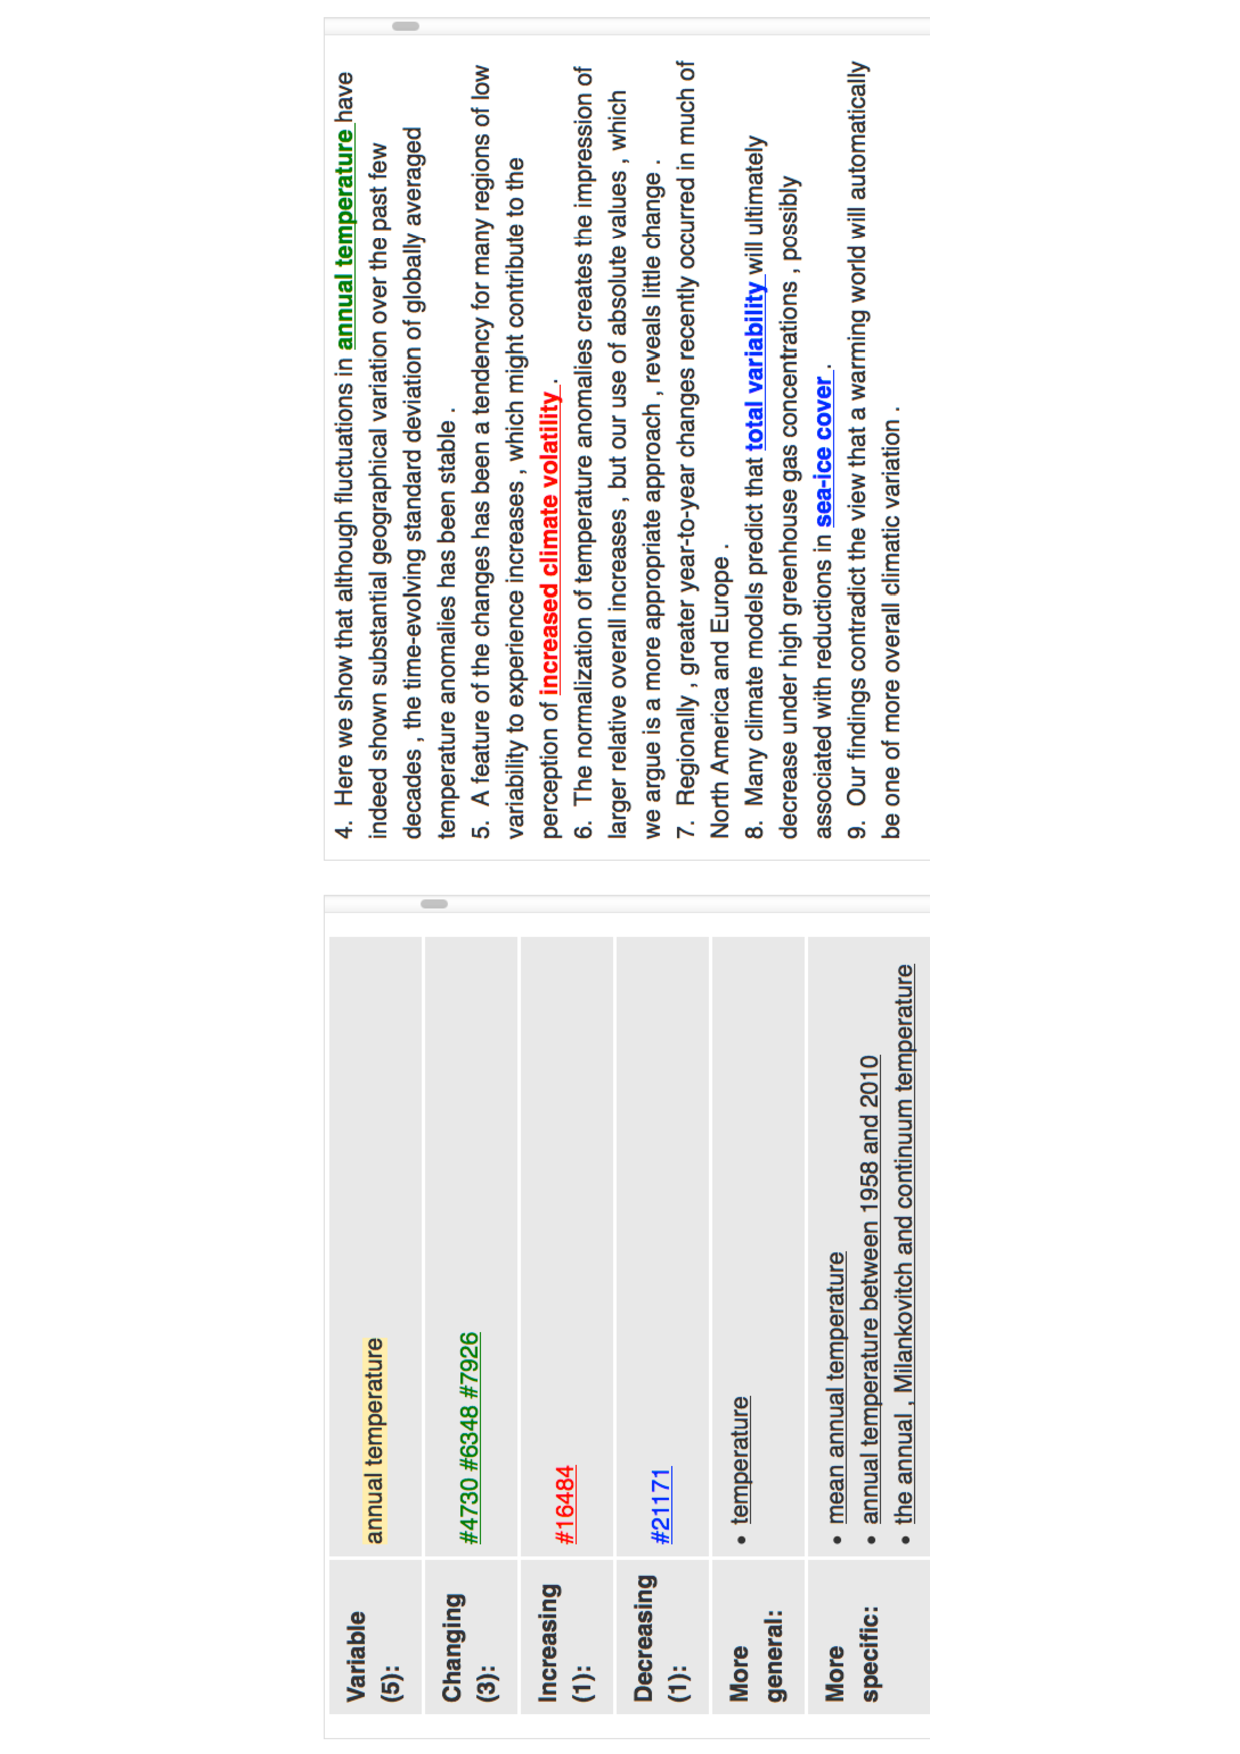
\includegraphics[angle=-90,width=0.5\textwidth,clip=true,trim=56mm 1mm 53mm 0]{screenshot.pdf}
\end{tikzfigure}

}	
    

    
     
\column{0.45}

%-----------------------------------------------------------------------------------
\block{Discussion}
%-----------------------------------------------------------------------------------    
{  
\begin{itemize}
\item \point{Parsing errors} (e.g. in coordination and PP-attachment) appear to be main source of extraction errors, because patterns fail to match or match unintentionally, yielding incomplete or incoherent variables 
\item \point{Limitations of pattern matching}
\begin{itemize}
\item pattern may have different semantics, e.g., \emph{change in western Europe}
\item change may be entailed, e.g. \emph{ocean acidification}, i.e. increase in acidity 
\item embedded variables, e.g. \emph{reduce subseasonal temperature variance}
\item negation, e.g. \emph{not decreasing}
\end{itemize}
\end{itemize}    
}

%-----------------------------------------------------------------------------------
\block{Ongoing/Future work}
%-----------------------------------------------------------------------------------    
{  
\begin{itemize}
\item \point{evaluation} of extractions and generalisations by domain experts
\item \point{association mining} from frequently co-occurring variables
\item \point{causal relation extraction} between changing variables
\item \point{scaling} to much larger data sets of full papers   
\end{itemize}    

}

\end{columns}

 
\end{document}

